\documentclass[11pt]{article}
\usepackage[utf8]{inputenc}
\usepackage{amsmath}
\usepackage{graphicx}
\usepackage{listings}
\usepackage{verbatim}
\usepackage{float}
\usepackage{xcolor}
\usepackage{subcaption}
\usepackage[english]{babel}
\usepackage{caption}
\usepackage{hyperref}
\usepackage{biblatex}
%\addbibresource{project2.bib}
\usepackage{setspace}
\usepackage{wrapfig}
\usepackage{lipsum}
\usepackage{amssymb}
\linespread{1.15}
\usepackage[a4paper, total={6.5in, 9in}]{geometry}
\DeclareMathOperator*{\E}{\mathbb{E}}


\hypersetup{
    colorlinks,
    linkcolor={red!50!black},
    citecolor={blue!50!black},
    urlcolor={blue!80!black}
}
\definecolor{codegreen}{rgb}{0,0.6,0}
\definecolor{codegray}{rgb}{0.5,0.5,0.5}
\definecolor{codepurple}{rgb}{0.58,0,0.82}
\definecolor{backcolour}{rgb}{0.95,0.95,0.92}
\definecolor{dkgreen}{rgb}{0,0.6,0}
\definecolor{gray}{rgb}{0.5,0.5,0.5}
\definecolor{mauve}{rgb}{0.58,0,0.82}

\lstdefinestyle{mystyle}{
    backgroundcolor=\color{backcolour},
    commentstyle=\color{codegreen},
    keywordstyle=\color{magenta},
    numberstyle=\tiny\color{codegray},
    stringstyle=\color{codepurple},
    basicstyle=\ttfamily\footnotesize,
    breakatwhitespace=false,
    breaklines=true,
    captionpos=b,
    keepspaces=true,
    numbers=left,
    numbersep=5pt,
    showspaces=false,
    showstringspaces=false,
    showtabs=false,
    tabsize=2
}

\lstset{style=mystyle}
\title{The Bias-variance-trade-off}
\author{Filip Severin von der Lippe}
\date{\today}
\begin{document}
\maketitle
GitHub repository containing code and further instructions on how to reproduce the results of this report: \url{https://github.com/Fslippe/FYS-STK4155/tree/main/project3/extra}

\section{Introduction}
In this report we will perform a bias-variance trade-off analysis of different methods. We will look at a regression problem using the well known Boston housing dataset which contains various parameters of the neighbourhood influencing the median value of owner-occupied homes. We will look into decision trees, starting with a single tree and move over to a random forest. A Feed forward Neural Network will also be studied. We will start off by introducing the theory behind the bias-variance trade-off and the methods used in the analysis before presenting and discuss the results of the different methods. In the end we will summarize our findings and propose possible further analysis.

\section{Method}
\subsection*{Bootstrap}

To study the bias-variance trade-off we first implement the bootstrap resampling technique. This is done by resampling our train data $n_B$ times with replacement. That means we gain $n_B$ new samples that may be unique but still only contain values from the original sample. This means that we can draw a sample from the original [1,2,3] to be for example [2,1,2]. For significant large amounts of training data, we are left with a minimal chance of drawing the same sample multiple times. From this we get by following the central limit theorem under the assumption that all our $n_B$ subsets are drawn from the same distribution, a normal distribution describing our data with original length $n$ with mean $\frac{1}{n}\sum_i y_i$
and standard deviation $\sigma/ \sqrt{m-1}$ for $m$ new data subsets and the original standard deviation of the distribution $\sigma$.
\subsection*{Bias-variance trade-off}
We define a cost function given by the mean squared error for a prediction vector $\tilde{\boldsymbol{y}}= \boldsymbol{X} \boldsymbol{\beta}$ and the true data vector $\boldsymbol{y}$.
\begin{align*}
    C(\boldsymbol{X}, \boldsymbol{\beta}) = \frac{1 }{n }\sum_ {i=0}^{n-1}(y_i - \tilde{y}_i)^2 = \E[(\boldsymbol{y}- \boldsymbol{\tilde{y}})^2]
\end{align*}
Here we have defined our dataset on the form $\boldsymbol{X} = (\boldsymbol{X}_j, y_j)$ for $j= 0, 1, ..., n-1$.
We continue by defining the input target data to be given by some function and noise $\epsilon\sim N(0, \sigma^2)$
\begin{align*}
    \boldsymbol{y} = f(\boldsymbol{x}) + \boldsymbol{\epsilon}.
\end{align*}

By the definition of our data $\boldsymbol{y} = f +\epsilon$ we rewrite the costfunction:
\begin{align*}
    \E[(\boldsymbol{y}- \boldsymbol{\tilde{y}})^2] & = \E[(f + \epsilon - \tilde{y} + \E[\tilde{y}]- \E[\tilde{y}])^2]                \\                                             &= \E[f^2 + \epsilon^2 + \tilde{y}^2 + 2\E[\tilde{y}]^2 \\
                                                   & + 2f\epsilon + 2f\tilde{y} + 2f\E[\tilde{y}] - 2f\E[\tilde{y}]                   \\
                                                   & + 2\epsilon\tilde{y} + 2\epsilon \E[\tilde{y}] - 2\epsilon \E[\tilde{y}]         \\
                                                   & + 2\tilde{y}\E[\tilde{y}] - 2\tilde{y}\E[\tilde{y}] -2\E[\tilde{y}]^2]           \\
                                                   & = \E[(f-\E[\Tilde{y}])^2] + \E[\epsilon^2] + \E[( \E[\Tilde{y}] - \Tilde{y} )^2] \\
                                                   & + 2(f-\E[\tilde{y}])\E[\epsilon]+2\E[\epsilon]\E[(\E[\tilde{y}]-\tilde{y} )]     \\
                                                   & + 2(f-\E[\tilde{y}])\E[( \E[\tilde{y}] - \tilde{y} )].
\end{align*}
By using that $\epsilon \sim N(0,1)$ we have $\E[\epsilon] = 0$ and Var$[\epsilon] = \E[\epsilon^2]- \E[\epsilon]^2 = \E[\epsilon^2]=\sigma^2$ from this we get:
\begin{align*}
    \E[(\boldsymbol{y}- \boldsymbol{\tilde{y}})^2] & =\E[(f -\E[\tilde{y}])^2] +\E[( \tilde{y} -\E[\tilde{y}])^2]  + \sigma^2+ 2(f-\E[\tilde{y}])\E[\E[\tilde{y}] -\tilde{y}] \\
                                                   & =\E[(f -\E[\tilde{y}])^2]  + \E[( \tilde{y} -\E[\tilde{y}])^2]+\sigma^2.
\end{align*}
Writing the expectation values in terms of the mean function $\E(\boldsymbol{x}) = \frac{1}{n}\sum_{i} x_i$, we get:
\begin{align*}
    \E[(\boldsymbol{y}- \boldsymbol{\tilde{y}})^2] & = \frac{1}{n}\sum_i (f_i - \E[\tilde{y}])^2 + \frac{1}{n} \sum_i ( \tilde{y}_i - \E[\tilde{y}])^2 + \sigma^2 \\ &= \quad\quad \text{Bias}^2 \quad\quad\quad + \quad \text{ Variance} \quad\quad + \quad \text{Noise}.
\end{align*}
We face a problem in the calculation of the bias because of the unknown $f_i$. To get around this we rewrite the bias term with help from the definition $\boldsymbol{y} = f + \boldsymbol{\epsilon}$.
\begin{align*}
    \E[y - \E[\tilde{y}]^2] & = \E[(f+\epsilon - \E[\tilde{y}])^2] = \E[\epsilon^2] + \E[(f - \E[\tilde{y}])^2] + \E[-2\epsilon(f- \E[\hat{y}])]        \\
                            & = \sigma^2 + \E[(f - \E[\tilde{y}])^2] + \E[-2\epsilon]\E[f-\E[\tilde{y}]] + \text{Cov}(-2\epsilon, (f- \E[\tilde{y}])^2) \\
                            & = \sigma^2 + \text{Bias}^2.
\end{align*}
In practice, this means that our calculated bias using $\boldsymbol{y}$ instead of $\epsilon$ has an error of $\sigma^2$. By assuming this error is very small will the new way of calculating the bias be very accurate.

\subsection*{Data}
The data we will use is the Boston housing set which can be loaded into python by scikit learn. The dataset contains 506 values for 13 features and one target feature as seen below in table \ref{tab:data}.
\begin{table}[H]
    \begin{small}
        \caption{The Boston housing dataset and its features.}
        \label{tab:data}
        \begin{center}
            \begin{tabular}{|l|l|}
                \hline
                \textbf{Feature} & \textbf{Desctiption}                                                     \\
                \hline
                CRIM             & per capita crime rate by town
                \\ \hline
                ZN               & proportion of residential land zoned for lots over 25,000 sq.ft.
                \\ \hline

                INDUS            & proportion of non-retail business acres per town
                \\ \hline

                CHAS             & Charles River dummy variable (= 1 if tract bounds
                river; 0 otherwise)
                \\ \hline

                NOX              & nitric oxides concentration (parts per 10 million)
                \\ \hline

                RM               & average number of rooms per dwelling
                \\ \hline

                AGE              & proportion of owner-occupied units built prior to 1940
                \\ \hline

                DIS              & weighted distances to five Boston employment centres
                \\ \hline

                RAD              & index of accessibility to radial highways
                \\ \hline

                TAX              & full-value property-tax rate per $10000 \$$
                \\ \hline

                PTRATIO          & pupil-teacher ratio by town
                \\ \hline

                B                & $1000(B_k - 0.63)^2$ where $B_k$ is the proportion of
                blacks by town
                \\ \hline

                LSTAT            & lower status of the population
                \\ \hline

                MEDV             & \textbf{Target data} - Median value of owner-occupied homes in $1000 \$$ \\
                \hline
            \end{tabular}
        \end{center}
    \end{small}
\end{table}

Since the bias-variance analysis can be computationally heavy, we sample only 202 random values from the original data. For this smaller dataset we perform a 80-20\% train-test split before standard scaling the data as
\begin{align*}
    y = \frac{y - \bar{y}_{train} }{\sqrt{\text{Var}({y_{train}})}} \quad \text{and}\quad \frac{\boldsymbol{X} - \bar{\boldsymbol{X}}_{train} }{\sqrt{\text{Var}({\boldsymbol{X}_{train}})}}.
\end{align*}

\subsection*{Regression methods}
\subsubsection*{Decision trees}
For a regression case a decision tree starts by looking at all possible values $x_1,x_2,...,x_p$ and making $J$ non overlapping regions around these. This means that we for new input data falling into a region $R_j$ will predict the value that initially made that region. The construction of the $J$ different regions are often not made exactly as described above, but made with a top-down approach. This means that we begin at the top of the tree and add to new branches corresponding to two new regions. We describe this in terms of a cutpoint $s$ splitting two regions $R_1$ and $R_2$ by
\begin{align*}
    \{X|x_j < s\} \quad\text{and}\quad \{X|x_j \geq s\}.
\end{align*}
Here we choose the feature $j$ and the cutpoint $s$ for the two regions based on the minimization of the $MSE$ for the input design matrix $X$ given by
\begin{align*}
    \sum_{i:x_i \in R_1} (y_i - \overline{y}_{R_1})^2  + \sum_{i:x_i \in R_2} (y_i - \overline{y}_{R_2})^2.
\end{align*}
This is done for every feature $p$ and every one of the $N$ data points, giving a total of $p \times N $ splits performed. The splitting process continues until all data has been classified, or until some stopping criteria such as a maximum depth of the tree or a minimum number of samples left in a leaf node. We will use the maximum depth of the tree as an adjustable parameter when we study the bias-variance trade-off. To generate the decision tree for our regression problem we use the DecisionTreeRegressor method from scikit learn.

\subsubsection*{Random Forest}
A big problem often found with a single decision tree is overfitting. This can be explained by how the tree can have almost an infinite number of branches, perfectly splitting up the training data to classify all the training samples. This can of course be solved by restricting the tree with for example a maximum depth, but also be solved by initializing several trees. We now have a forest of trees where each of them are trained on different subsets of data. These data subsets are made through bootstrapping of the training data. The branch splitting is done differently in a random forest. Here we select $m \leq p$ random variables from the $p$ predictors to consider for each split. This leaves us with trees that may look quite different from each other, because of the strongest predictors not always being among the $m$ variables, leaving us with these predictors not always being in the upper branches. The average of every tree's prediction is what leaves us with the final prediction. The random forest we will also be implemented through scikit learn with the method RandomForestRegressor, and we will look at how the tree depth and the number of trees influence the bias-variance trade-off.

\subsubsection*{Feed forward Neural Network}
A full description of a Feed Forward Neural Network (FFNN) can be found in \href{https://github.com/Fslippe/FYS-STK4155/blob/main/project2/latex/project2.pdf}{project 2}.


A FFNN is built up by layers of neurons each connected to every neuron of the neighbouring layers. Each neuron have its corresponding bias, and each connection have its own corresponding weight. These are respectively added and multiplied to the neurons input, and through backpropagation they are optimized to minimize some cost function to make better predictions. We will implement the FFNN with tensorflow sequential and look at both how different number of layers and neurons influence the bias-variance trade-off.

\section{Results and discussion}
\subsection*{Decision Tree}
For the decission tree we perform the bias-variance trade-off for 100 bootstrap samples and different number of tree depths up to a max depth of 20 as seen in figure \ref{fig:DT}.
\begin{figure}[H]
    \centering
    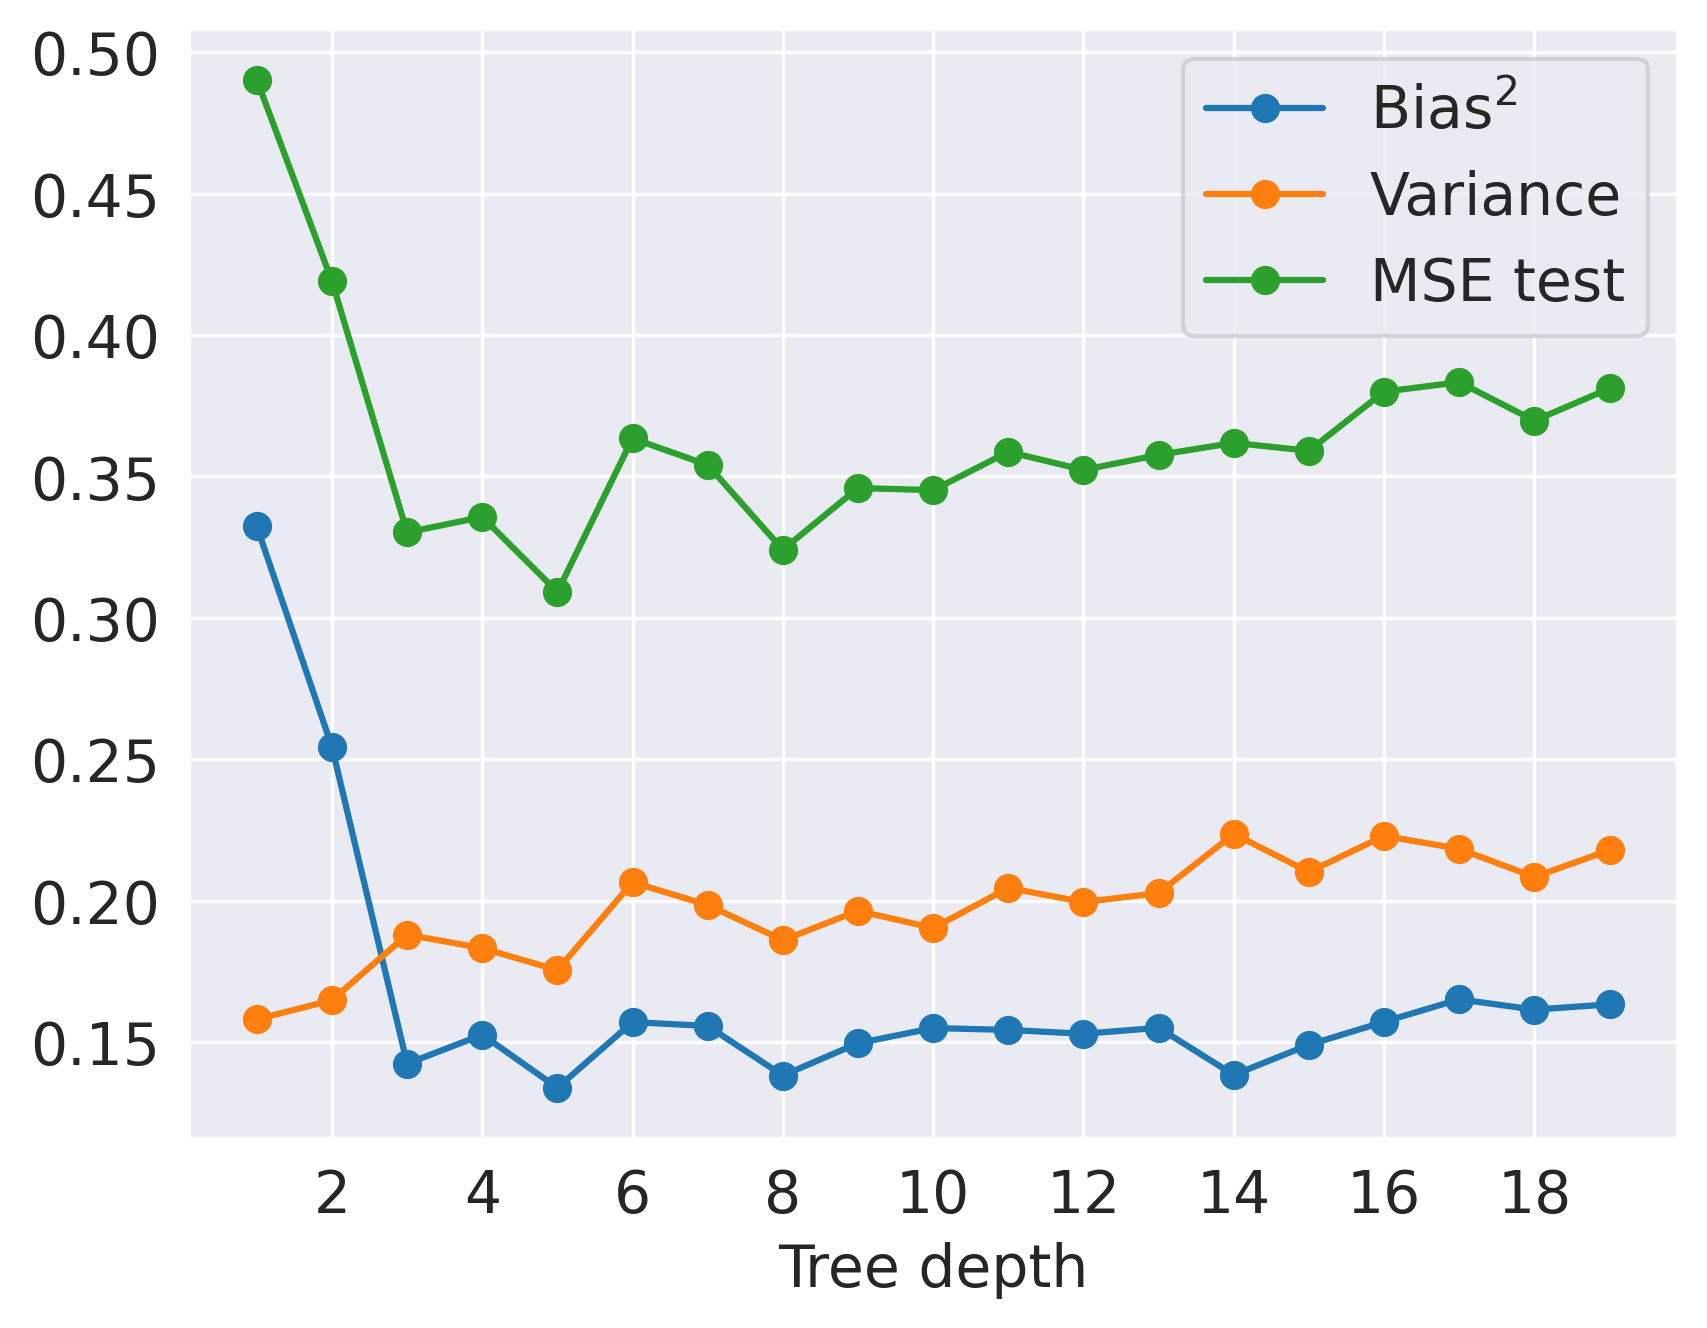
\includegraphics[width=0.5\textwidth]{figures/tradeoff_DT.png}
    \caption{Bias-variance trade-off as a function of maximum tree depth for a decision tree using 100 bootstrap samples.}
    \label{fig:DT}
\end{figure}
In figure \ref{fig:DT} we see that an increasing tree depth results in a decrease in the bias at the same time as an increase in the variance. Both of these contributions r results in the lowest mean squared error for a tree depth of 5 of 0.3. We see that also the bias starts increasing after this depth, indicating that we will not find a better prediction for a larger tree depth.
\subsection*{Random Forest}
Below in figure \ref{fig:RF} we see the bias-variance trade-off as a function of tree depth. We see 4 plots corresponding to different number of trees. We have again used 100 bootstrap samples.

There are small variations in the trade-off, and we mainly see a big drop in the MSE and bias when increasing the tree depth from 1 to 3. We notice that the bias is the main contributor to the MSE, also for larger tree depths. The variance stays small with only a small decrease by increasing the tree depth. We generally find the lower values of MSE from a decrease in bias for tree depths of 35 and above. This indicates that we may find even lower MSE by increasing the tree depth further. We notice almost no difference between different number of trees, but the overall lowest MSE is found by using 10 trees and a tree depth of 35. Compared to a single decision tree we see a much lower MSE of 0.15, which mainly comes from the much lower variance (0.05) since the biases have similar values (0.15).
\begin{figure}[H]
    \begin{subfigure}{.5\textwidth}
        \centering
        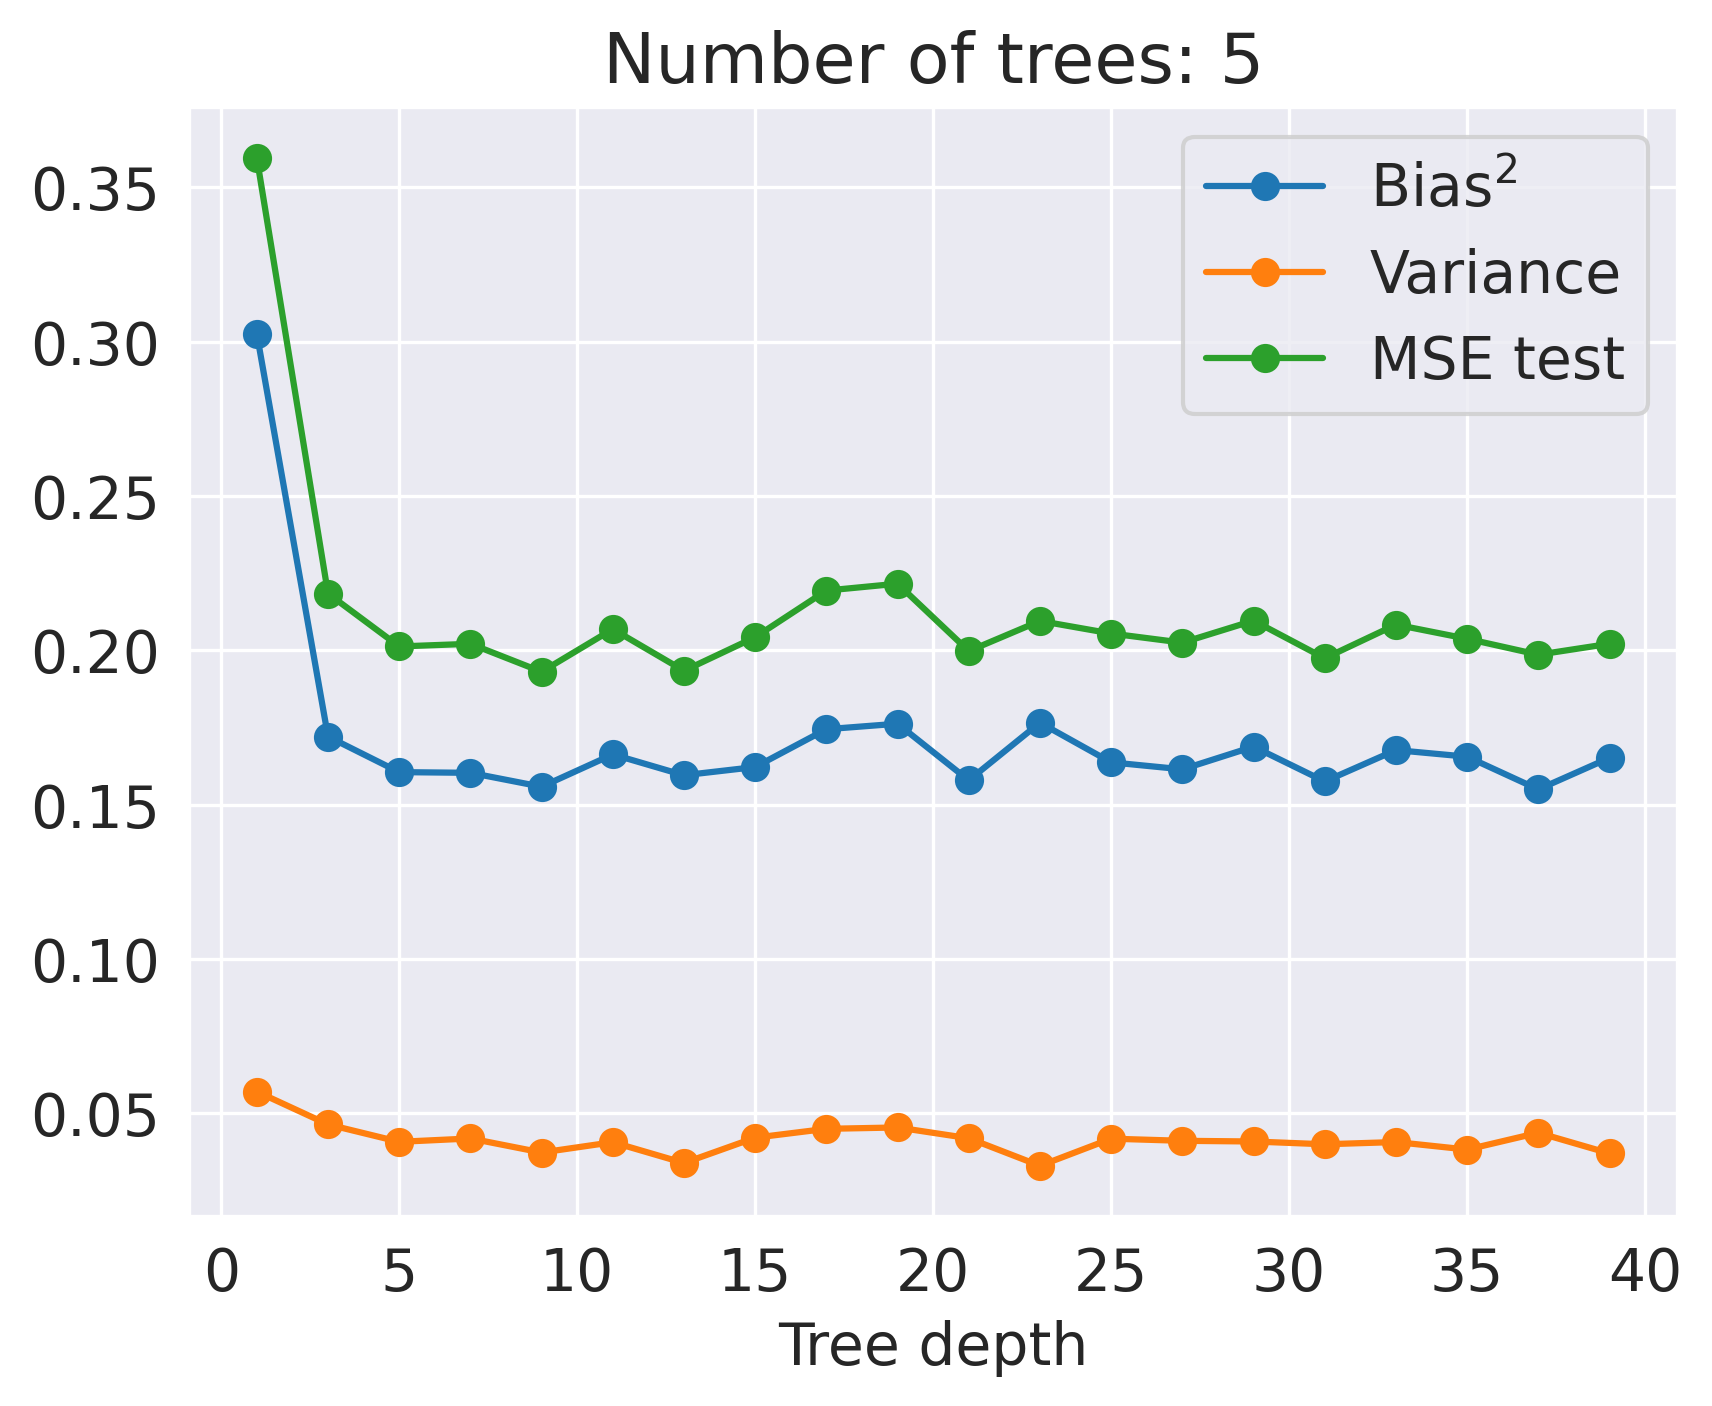
\includegraphics[width=.9\textwidth]{figures/tradeoff_RF_trees_5.png}
        \label{fig:}
    \end{subfigure}
    \begin{subfigure}{.5\textwidth}
        \centering
        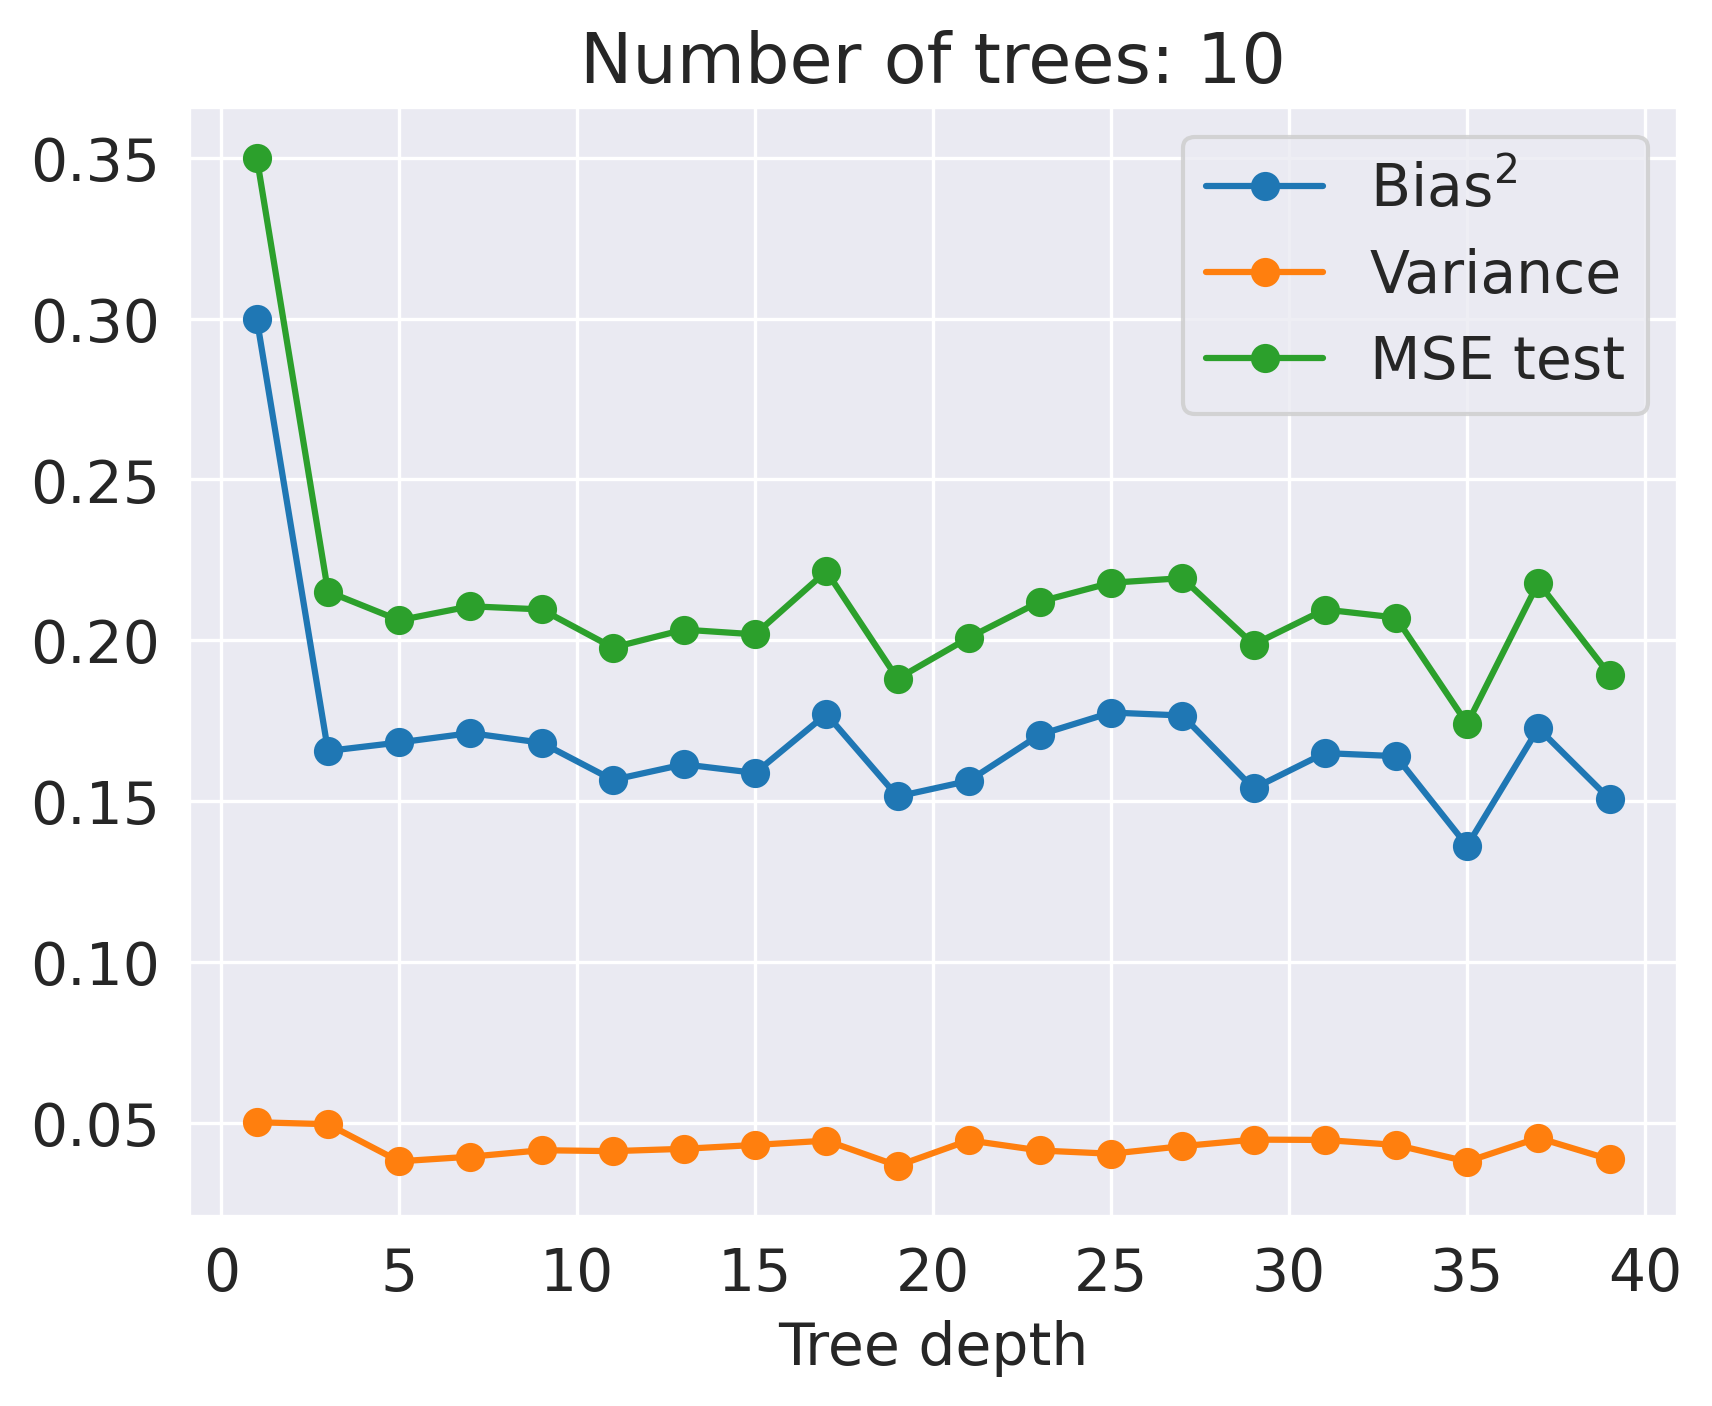
\includegraphics[width=.9\textwidth]{figures/tradeoff_RF_trees_10.png}
        \label{fig:}
    \end{subfigure}
    \begin{subfigure}{.5\textwidth}
        \centering
        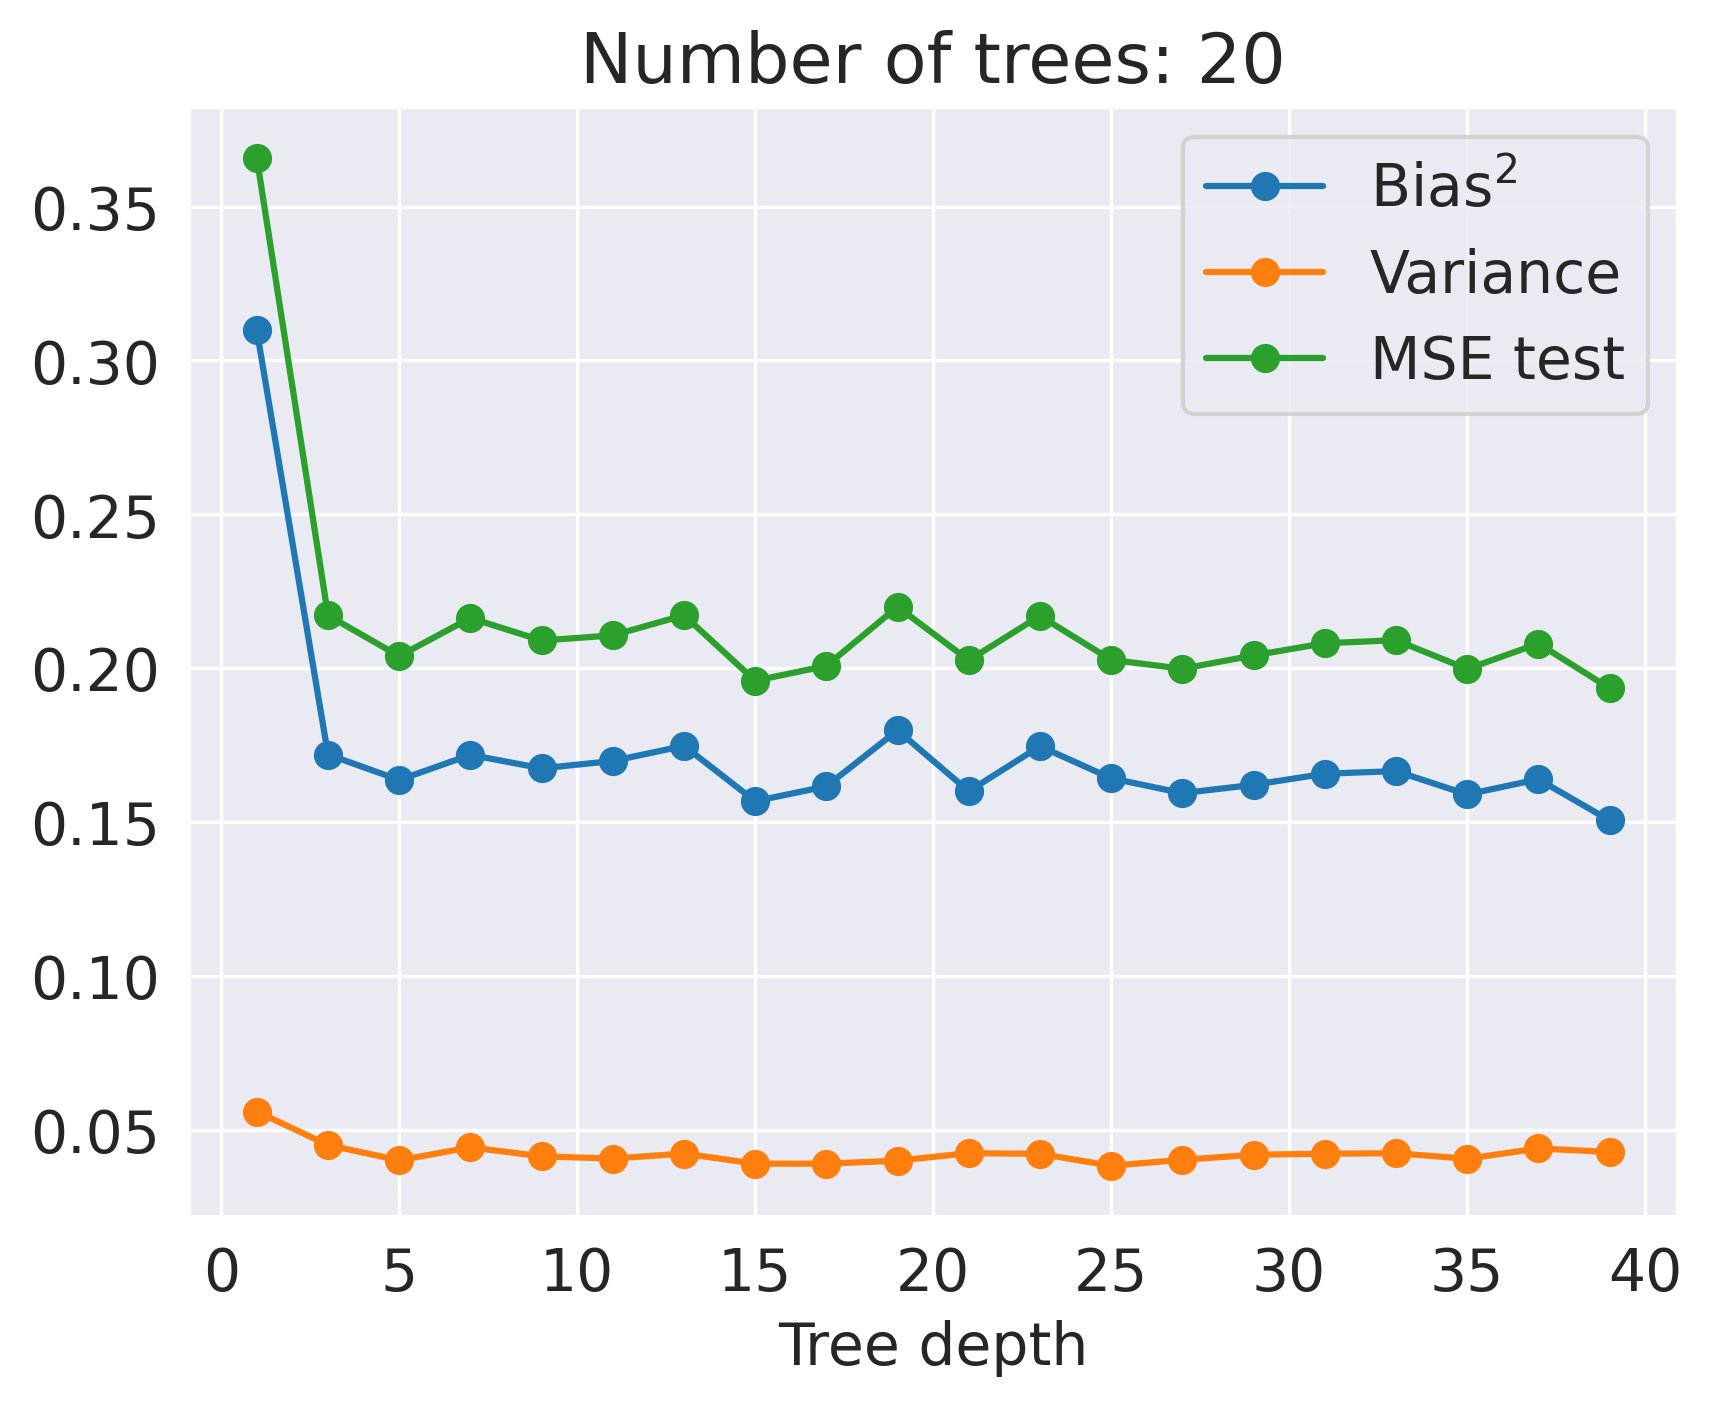
\includegraphics[width=.9\textwidth]{figures/tradeoff_RF_trees_20.png}
        \label{fig:}
    \end{subfigure}
    \begin{subfigure}{.5\textwidth}
        \centering
        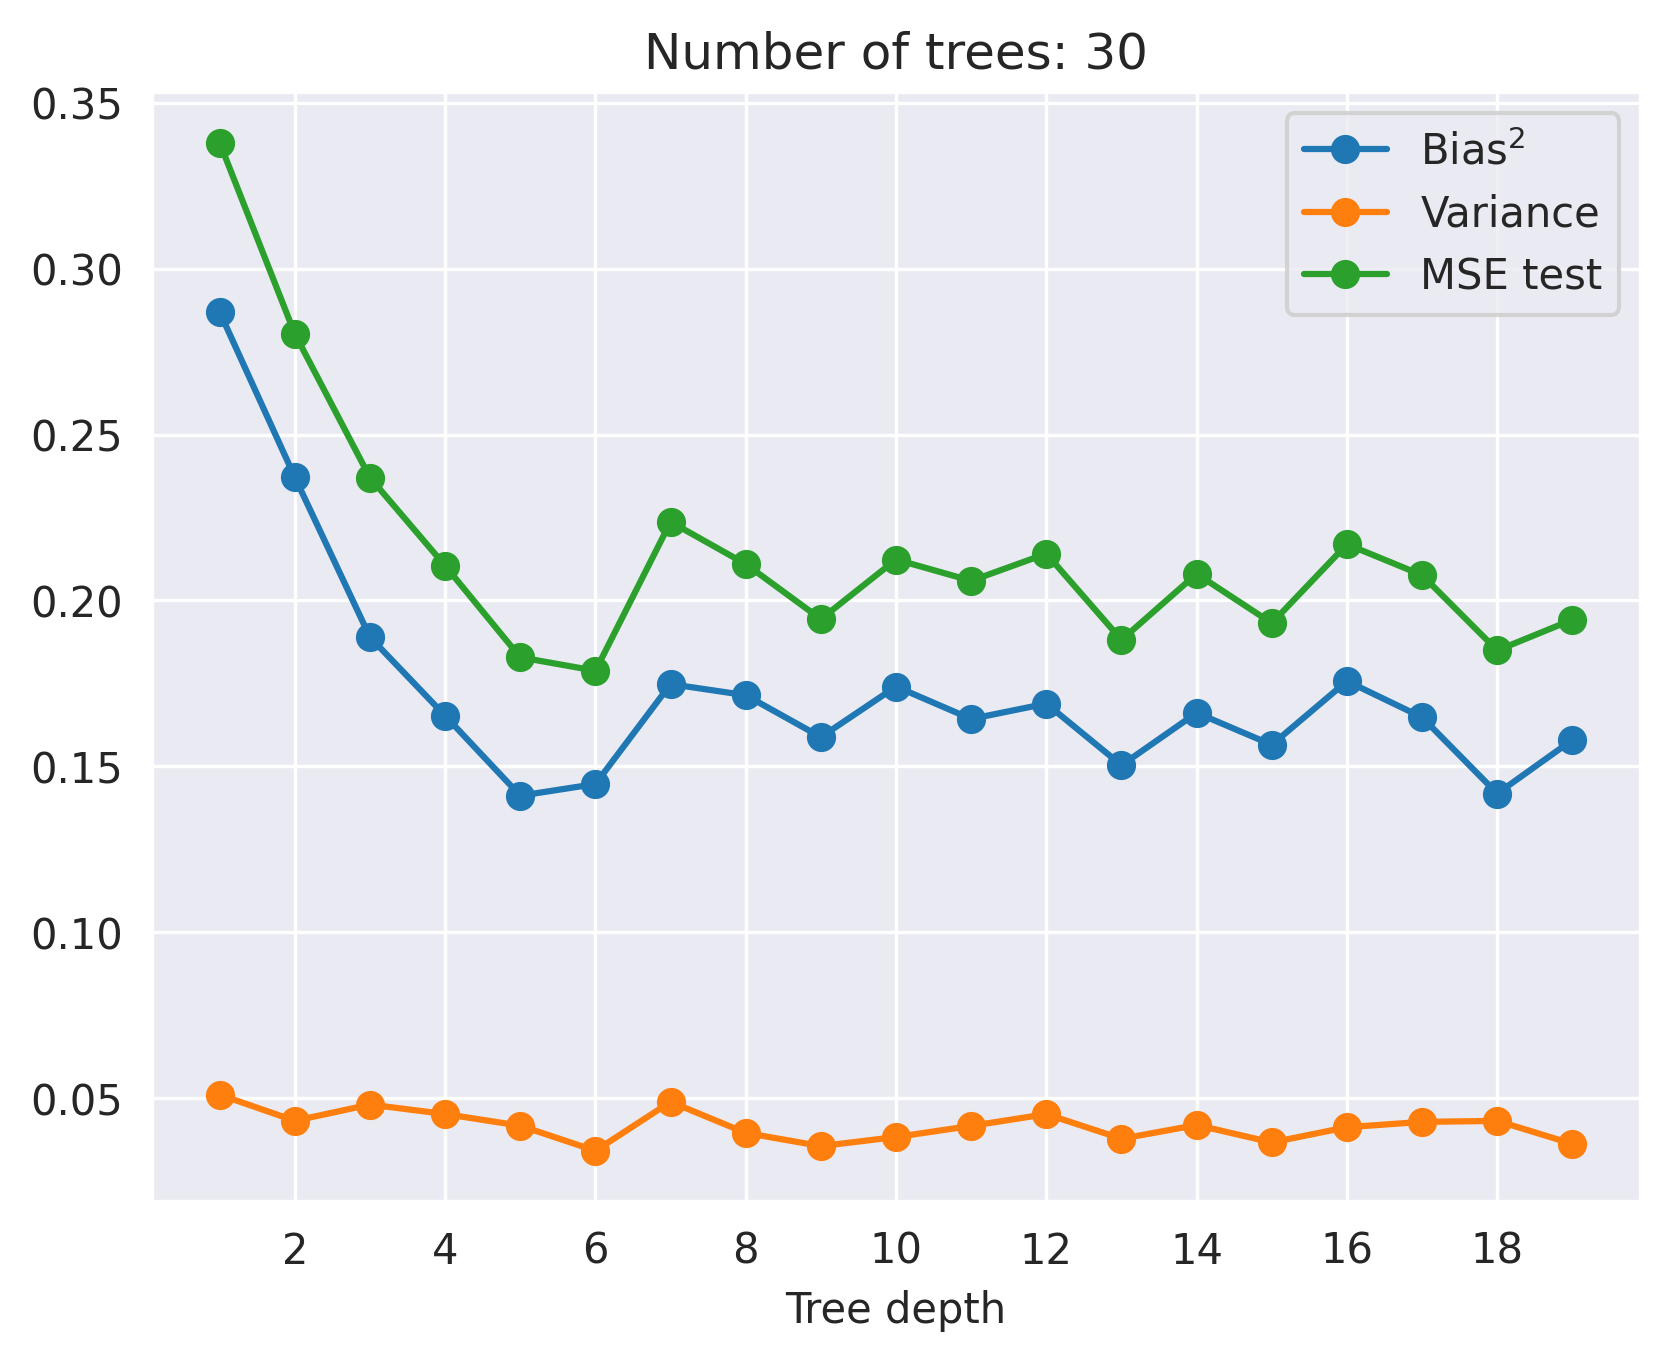
\includegraphics[width=.9\textwidth]{figures/tradeoff_RF_trees_30.png}
        \label{fig:}
    \end{subfigure}
    \caption{The bias-variance trade-off using 100 bootstrap samples as a function of tree depth up to a depth of 40 where every second tree depth is skipped. We see 4 plots corresponding to different number of trees in the forest. }
    \label{fig:RF}
\end{figure}

\subsection*{Feed Forward Neural Network}
In figure \ref{fig:NN} we see the bias-variance trade-off using 100 bootstrap samples for different number of neurons per layer. We see 4 plots corresponding to 1, 2, 3 and 4 layers in the neural network.

The 4 plots in figure \ref{fig:NN} all show quite varying results for different number of neurons, but we still notice a general trend. For all plots we see small variances between 0 and 1. We also see an increasing variance until around 10 neurons where a further increase generally equals a lower variance going towards 0. This shows that the bias is the main contributor to the MSE especially for a higher number of neurons. For 4 layers we see an indication of overfitting with a slight increase in the variance and MSE for higher number of neurons. In the other cases we see decreasing MSE for more neurons indicating that a further neuron increase could equal an even lower MSE. We see that the Neural Network have smaller MSE for certain number of neurons than both the decision tree and the random forest. We see MSE at or below 0.15 for all the tested number of layers, and even MSE below 0.1 for 2 layers and 58 neurons, and 4 layers and 21 neurons.
\begin{figure}[H]
    \begin{subfigure}{.5\textwidth}
        \centering
        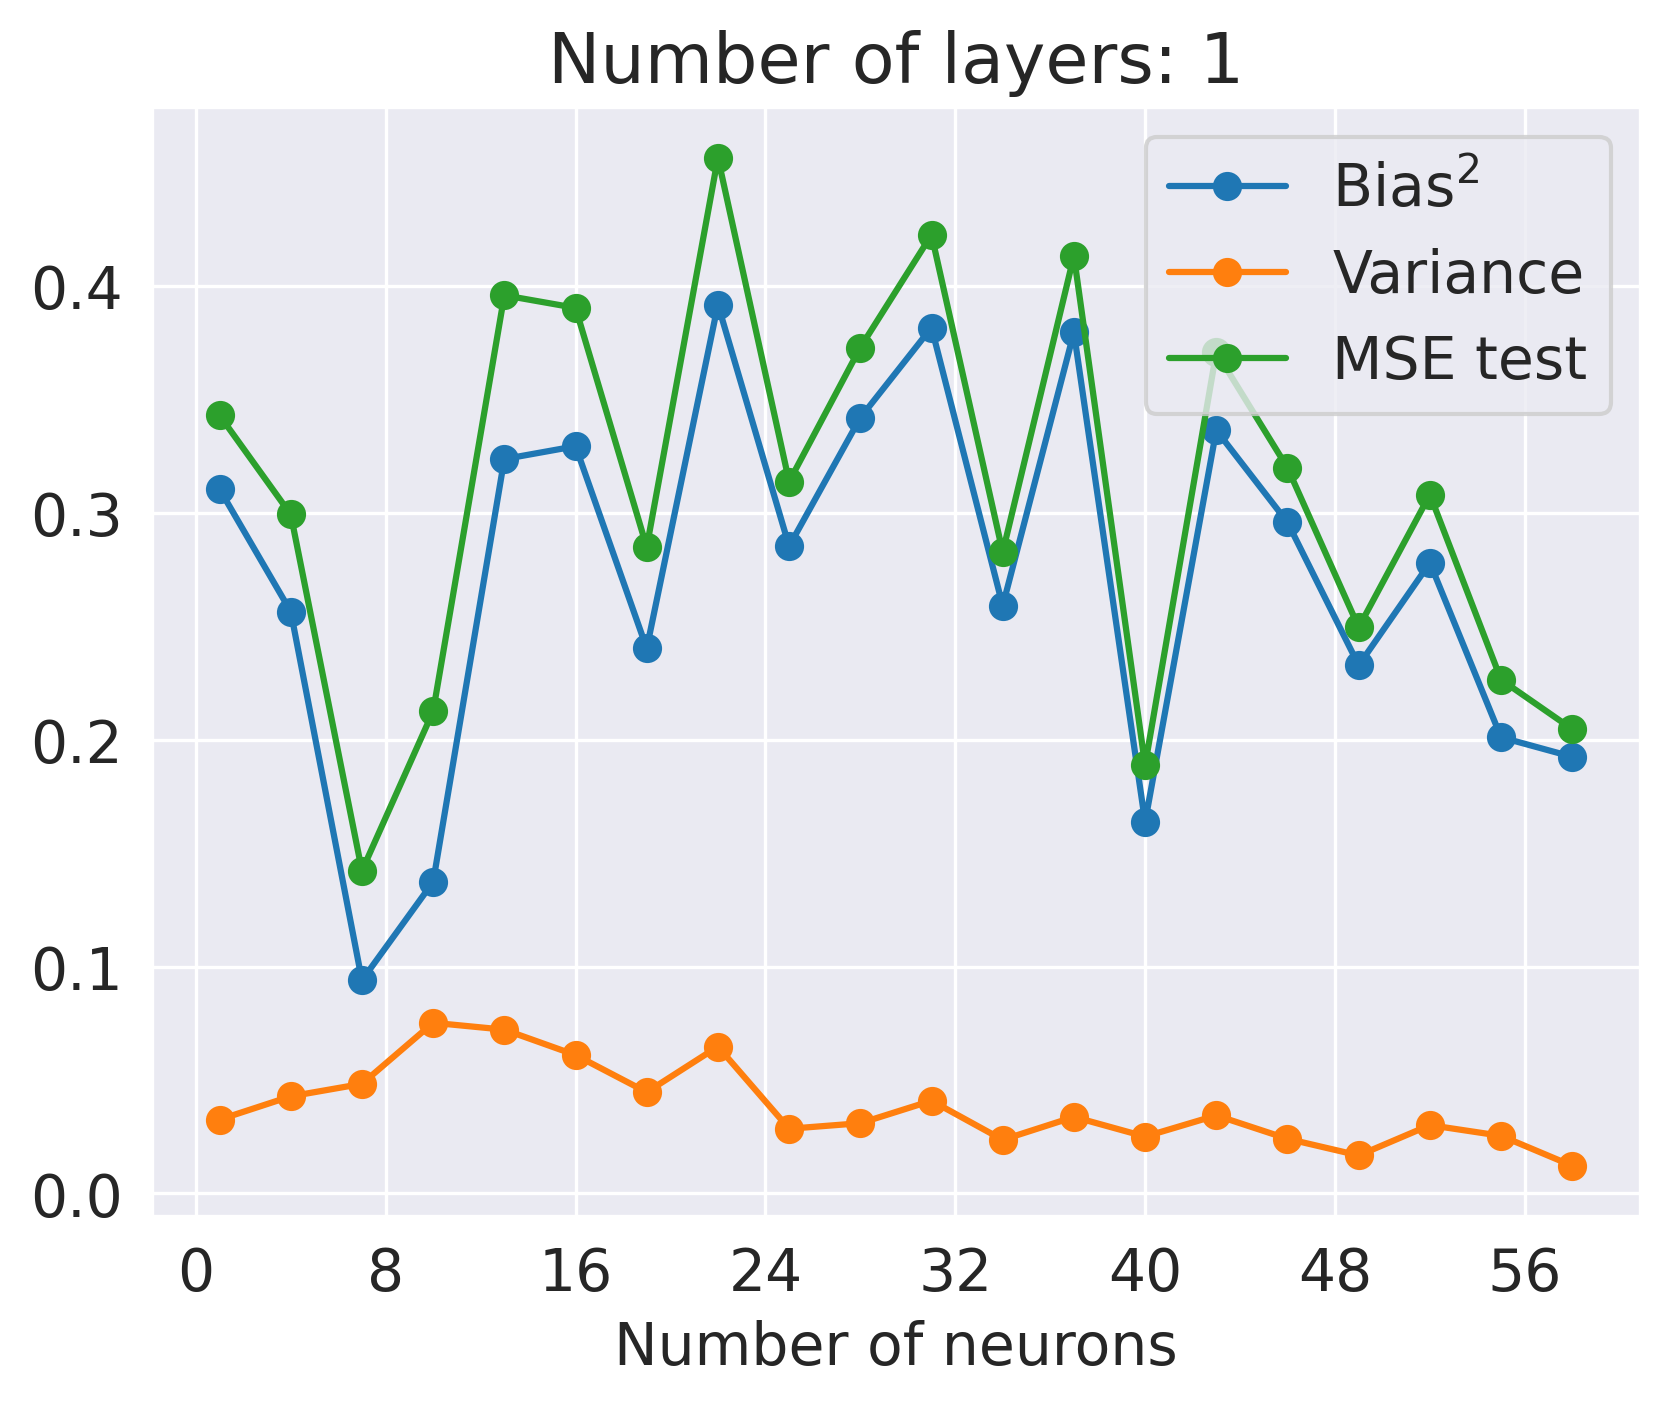
\includegraphics[width=.9\textwidth]{figures/tradeoff_NN_neurons_1.png}
        \label{fig:}
    \end{subfigure}
    \begin{subfigure}{.5\textwidth}
        \centering
        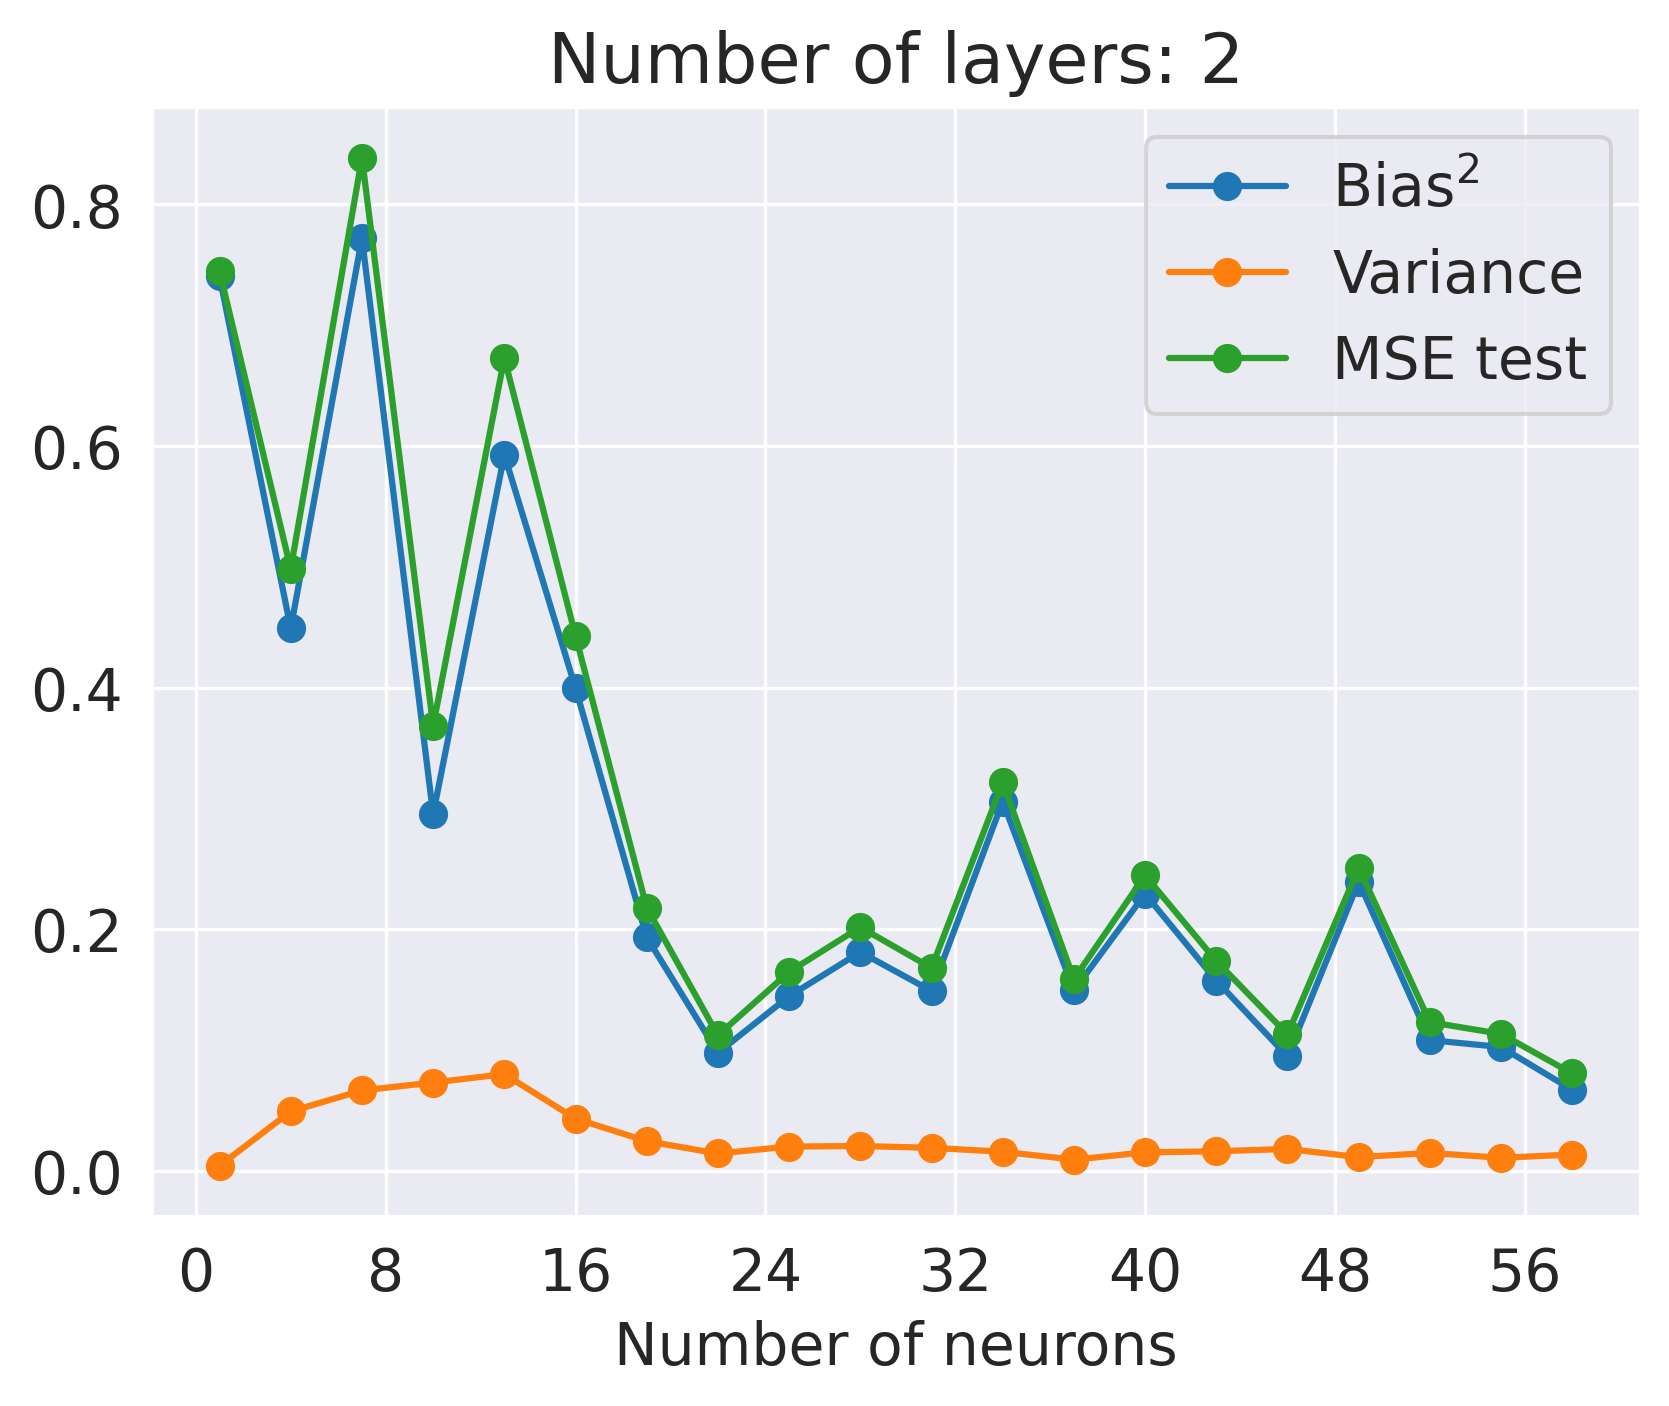
\includegraphics[width=.9\textwidth]{figures/tradeoff_NN_neurons_2.png}
        \label{fig:}
    \end{subfigure}
    \begin{subfigure}{.5\textwidth}
        \centering
        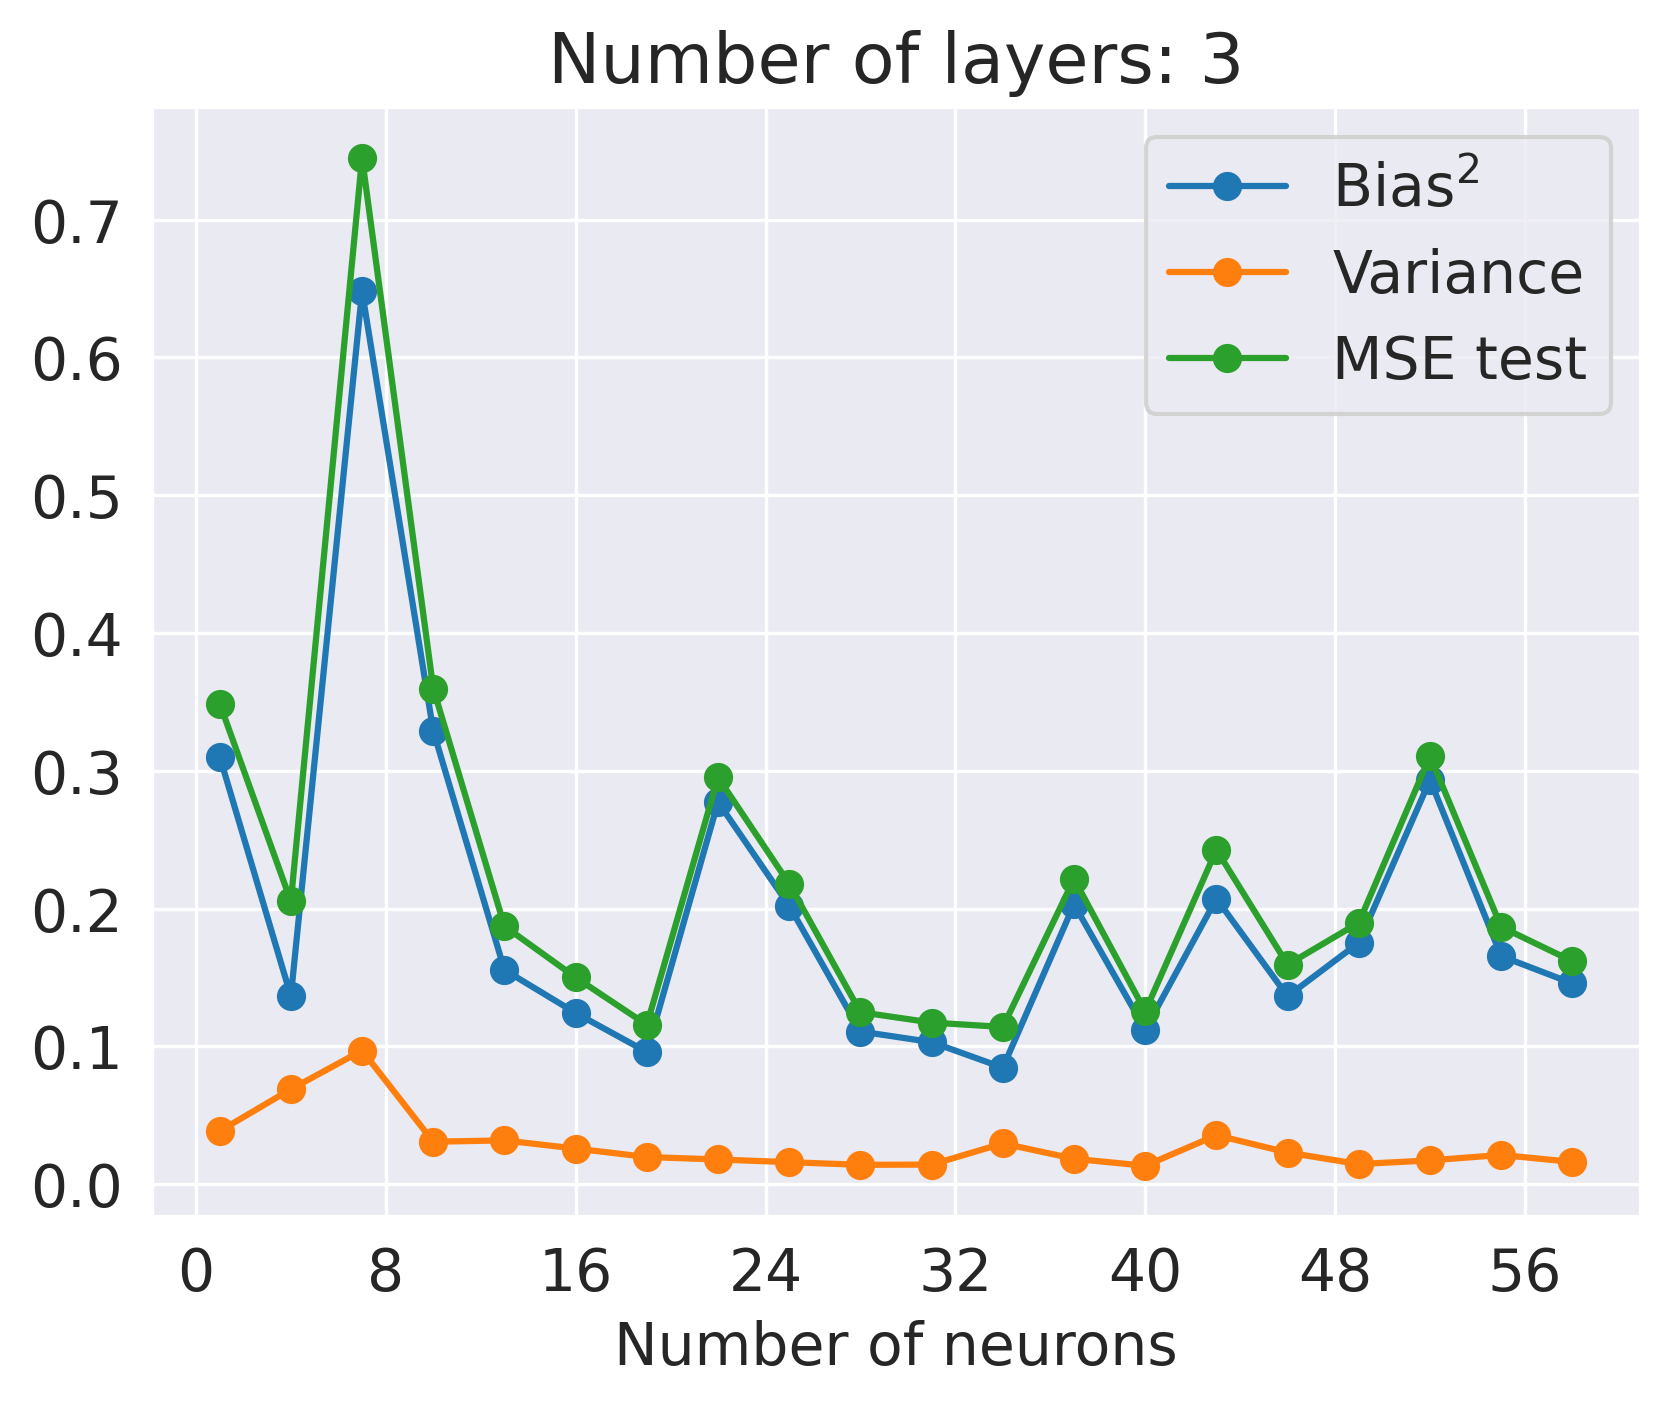
\includegraphics[width=.9\textwidth]{figures/tradeoff_NN_neurons_3.png}
        \label{fig:}
    \end{subfigure}
    \begin{subfigure}{.5\textwidth}
        \centering
        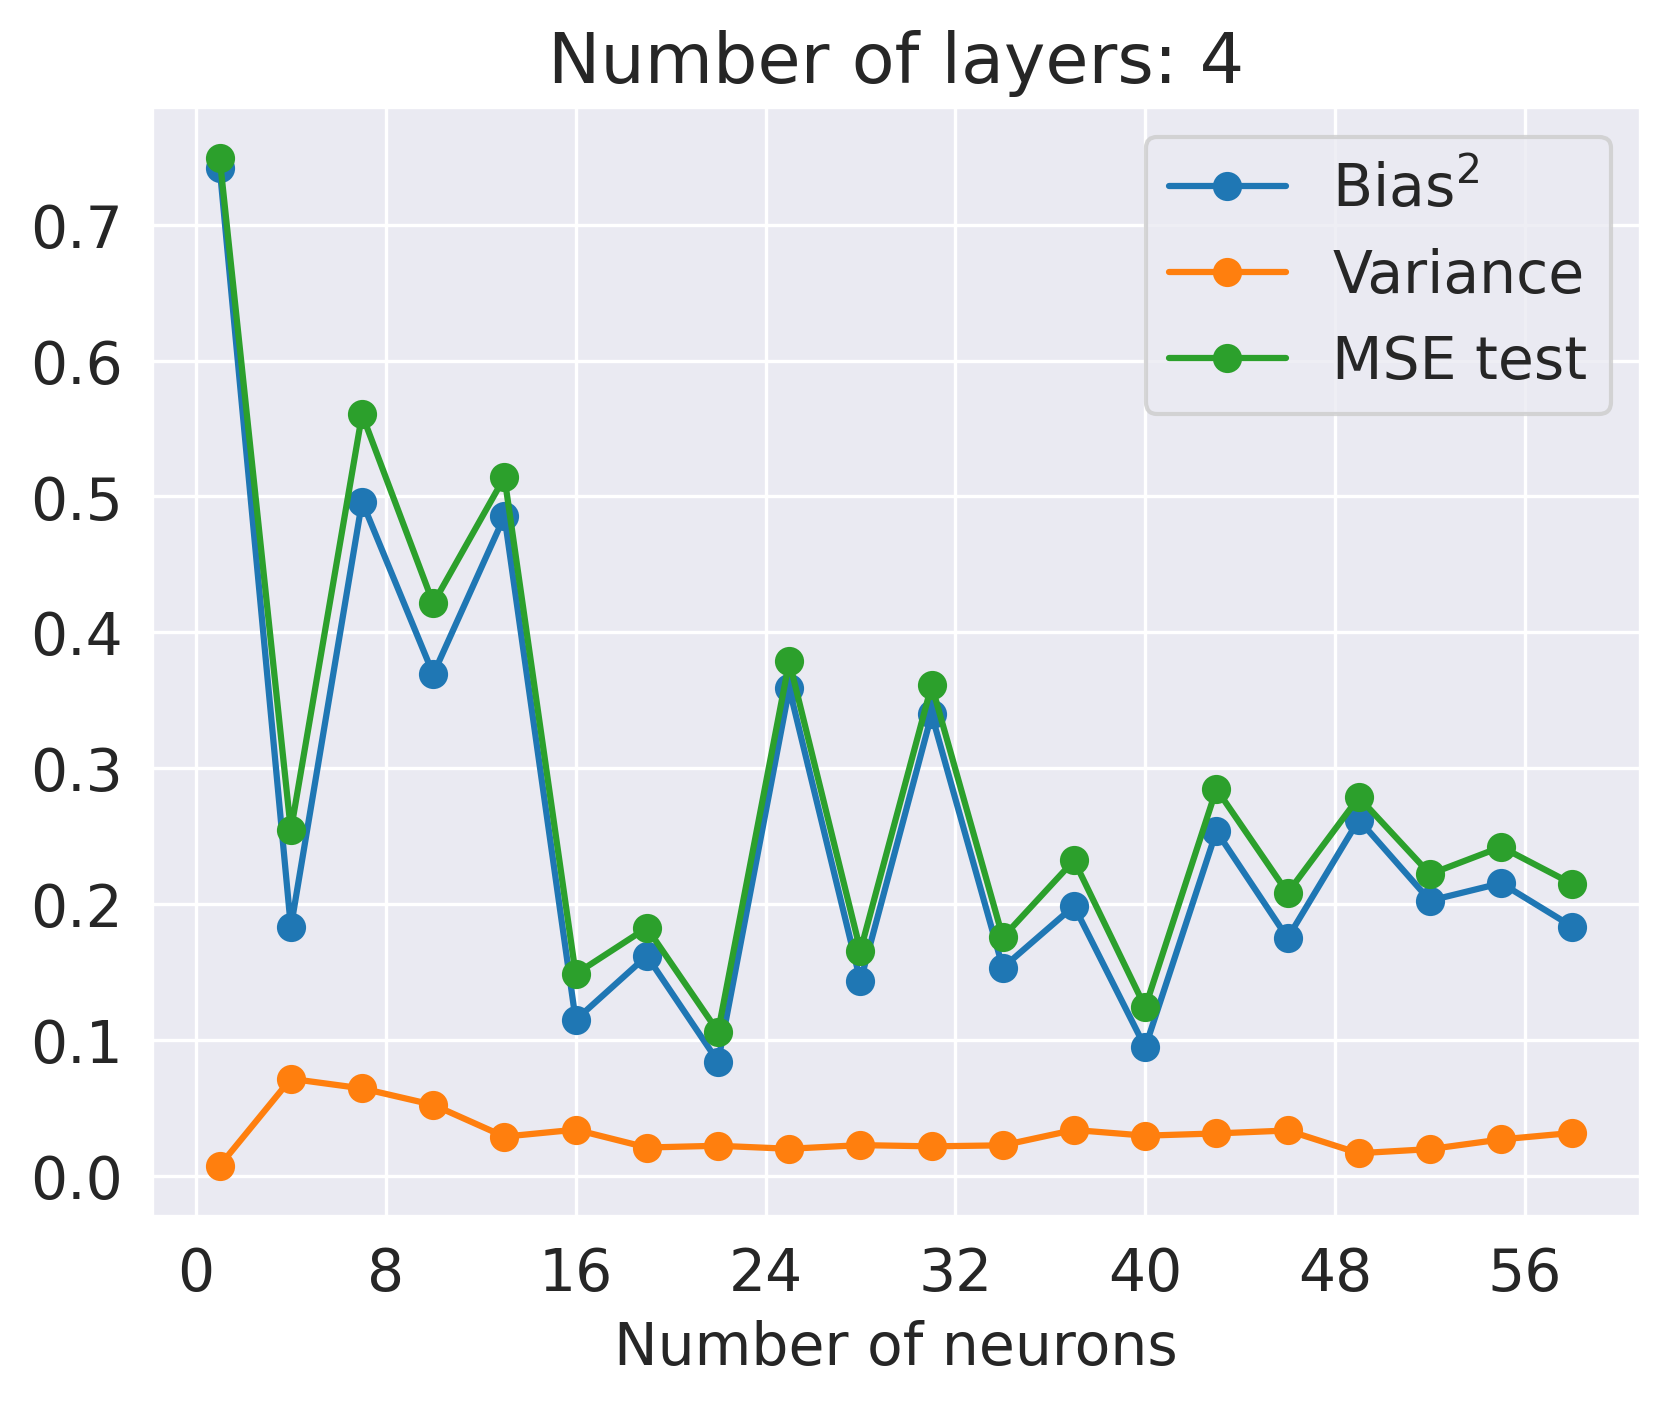
\includegraphics[width=.9\textwidth]{figures/tradeoff_NN_neurons_4.png}
        \label{fig:}
    \end{subfigure}
    \caption{The bias-variance trade-off using 100 bootstrap samples as a function of neurons in each layer up to a total of 58 neurons where every third neuron is skipped. We see 4 plots corresponding to different number of layers in the neural network.}
    \label{fig:NN}
\end{figure}

\section{Conclusion}
We have found that different methods and their different parameters equals very different bias-variance trade-offs. A single decision tree has shown the worst overall performance with a minimum MSE of 0.3. It had a more typical trade-off than the other methods with an increasing variance and decreasing bias for higher complexities. The random forest gave us very stable trade-offs with a small to no dependency on the number of trees. We saw no indication of overfitting. The bias was the main contributor to the MSE and its minimum of 0.15, and the variance stayed generally low. For the neural network we saw a quite varying trade-off with the bias being the main contributor to the MSE. We saw again no sign of overfitting except by using 4 layers with a slight increase in variance for higher number of neurons.
\end{document}